\documentclass[a4wide]{report}

\usepackage{amsmath}
\usepackage[a4paper, total={7in, 10.2in}]{geometry}
\usepackage{graphicx}
\usepackage[portuguese]{babel}
\usepackage[utf8]{inputenc}

\begin{document}

\noindent
{\bf Lincoln Martins de Oliveira (ES 90693) - Mini-relatório 02 (\today)}

\begin{quote}

\centering

\bf Mini relatório referente ao exercício 1 das aulas 9 e 10

\end{quote}
\vspace{0.5cm}


      Este exercício nos apresenta o metodo Newton-Raphson (veja pags 3 a 5 de ~\cite{Metodos}) que utilizamos para realizar
a implementação de um programa que através de um chute inicial do valor de x, isto é, a partir da escolha de um $x_0$ podemos 
encontrar as raizes de funções quaisquer, porem deve-se prestar bastante atenção nos valores de  $x_0$ escolhidos pois alguns 
podem dar algum problema. 


\begin{quote}


\bf 01) a e b-

\end{quote}

Nesta letra assumimos o que foi proposto por~\cite{roteiro} e fizemos um programa que se encontra na pasta $ex 01 a e b$ que calcula as
raizes da função $ f(x) = (3 + x)^2 - 12$. Tais raizes são respectivamente:

\begin{equation}
\centering
R_1= 0.46410161513775433    
\label{raiz1}
\end{equation}
\begin{equation}
\centering
R_2= -6.4641016151377544     
\label{raiz2}
\end{equation}

Observe que dentro do intervalo proposto por~\cite{roteiro} não podemos assumir $x_0 = -3$, 
pois deste modo a derivada seria zero e consequentemente o programa daria erro.

Plotamos o gráfico da f(x) para comparar com as raizes abaixo:
\begin{figure}[h]
\centering
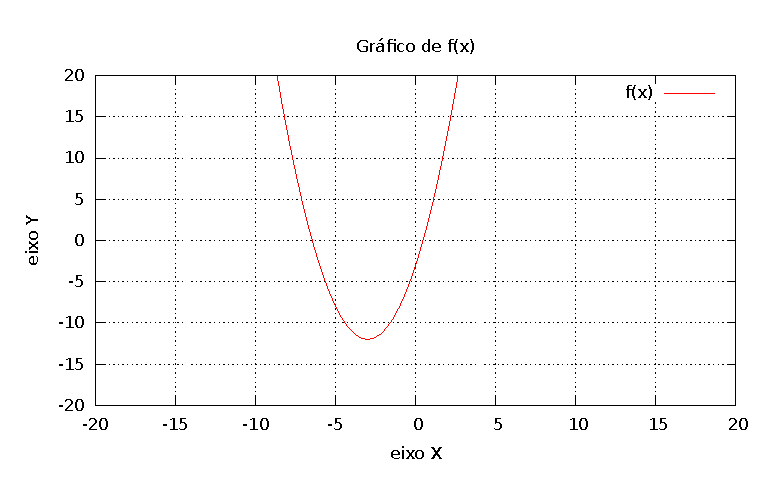
\includegraphics[width=0.5\textwidth]{grafico_ex_01_a}
\caption{Comportamento de f(x).}
\label{ex01a1.1}
\end{figure}

Plotamos também o gráfico~\ref{ex01a1.2} de n vs $x_n$  para vermos o que acontecia com os valores de n e $x_n$ a medida que o programa rodava:
\begin{figure}[h]
\centering
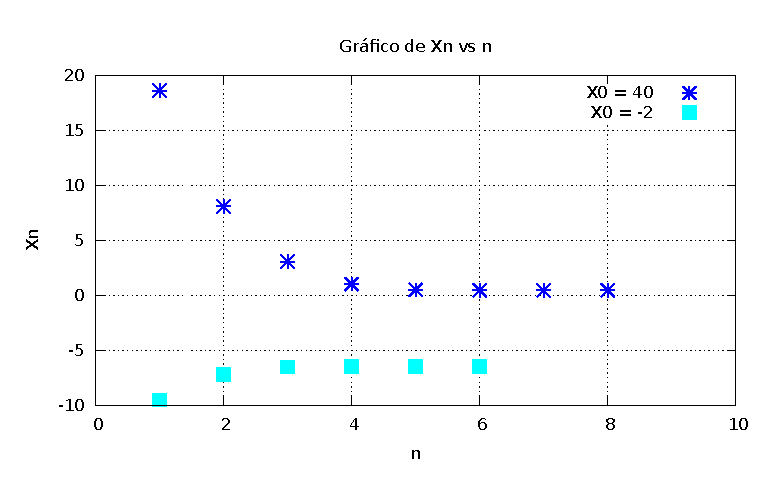
\includegraphics[width=0.6\textwidth]{grafico_do_ex01a_x=40_e_x0-2}
\caption{n vs $x_n$.}
\label{ex01a1.2}
\end{figure}
\\
\\
\\
\\
\\
\begin{quote}

\bf 01) c-

\end{quote}

Usando os valores proposto pelo item c de~\cite{roteiro} e a função $g(x) = [1 + (1 + x^2 )sen(x/5)]/(1 + x^2 )$ 
dentro do intervalo proposto em~\cite{roteiro}, foi feito um programa parecido com o do item a, para encontrar as raizes de g(x). 
Este programa se encontra na pasta $ex01c$, e os valores das raizes obtidas estão na tabela~\ref{intervalosraizes} abaixo com seu respectivo intervalo 
de $x_0$.

\begin{table}[!h]
\centering
 \begin{tabular}{cc}
  \hline\\[-0.37cm]
  \hline
      Intervalo       &   Raiz          \\ \hline
  -30 $<$ $x_0$ $<$ -23      &  -31.390086063181769     \\
  -22 $<$ $x_0$ $<$ -16      &	-15.691588937456128                 \\
 -6 $<$ $x_0$ $<$ -1       &    -1.5258651659857210          \\
 9 $<$ $x_0$ $<$ 15         &	    15.724208335212186               \\
 33 $<$ $x_0$ $<$ 40            &	31.441920337777852      \\
 \hline\\[-0.37cm]
  \hline
\end{tabular}
\caption{Raizes de $x_0$ para o intervalo determinado.}
\label{intervalosraizes}
\end{table}

Observe que os intervalos determinados na tabela~\ref{intervalosraizes} foram determinados observando 
o gráfico~\ref{ex01a1.3}  e vendo onde cada raiz estava aproximadamente.
\\
\\
\\
\\
\\

\begin{figure}[h]
\centering
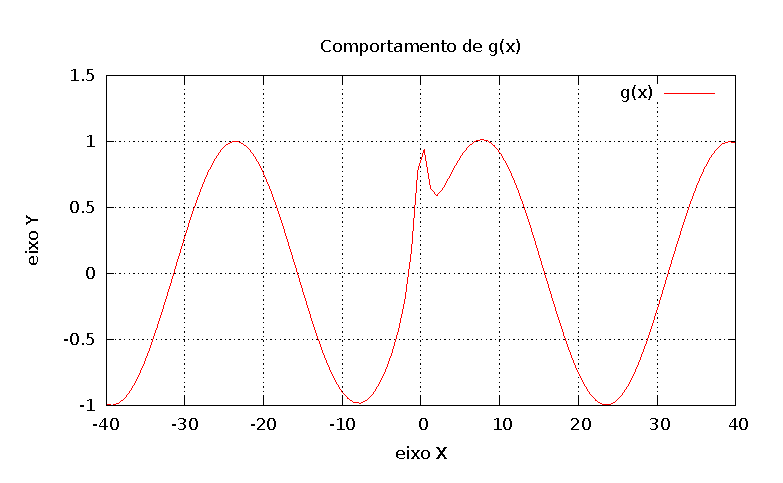
\includegraphics[width=0.5\textwidth]{teste}
\caption{Gráfico referente ao comportamento de g(x).}
\label{ex01a1.3}
\end{figure}
\begin{quote}

\bf 01) d-

\end{quote}

No item d fizemos um programa considerando a mesma função do item c, e computamos o número de passos n
necessários para que a solução convirja assumindo valores iniciais $x_0 = -2$, $x_0 = -3$ e $x_0 = -4$.
O programa referente a este item esta na pasta $ex01d$.

Os três Gráficos de n vs $x_n$ estão abaixo e mostram o número de vezes que o programa teve que rodar ate 
encontrar um valor satisfatório para a raiz:

\begin{figure}[h]
\centering
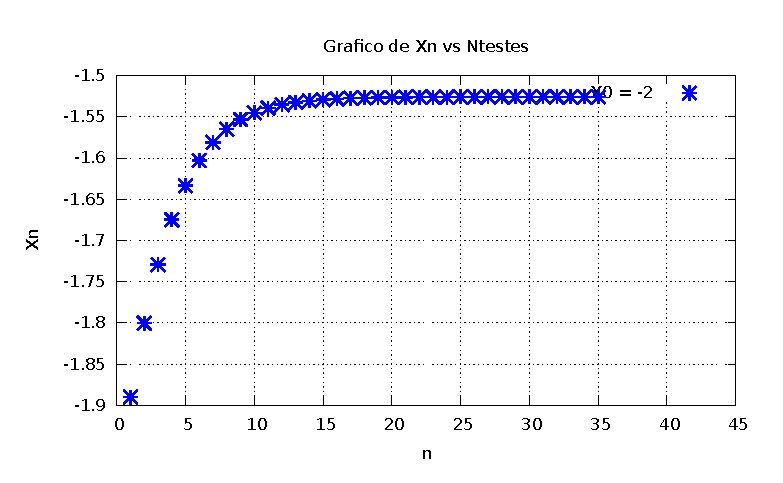
\includegraphics[width=0.5\textwidth]{grafico_do_ex01d_x=-2}
\caption{Gráfico representa o número de vezes que o programa rodou ate encontrar a raiz, para $x_0 = -2$.}
\label{ex01a1.4}
\end{figure}
\begin{figure}[h]
\centering
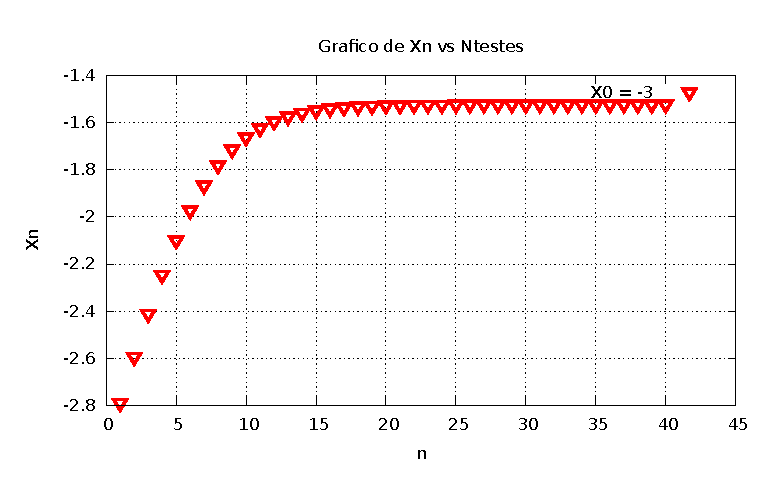
\includegraphics[width=0.5\textwidth]{grafico_do_ex01d_x=-3}
\caption{Gráfico representa o número de vezes que o programa rodou ate encontrar a raiz, para $x_0 = -3$.}
\label{ex01a1.5}
\end{figure}
\begin{figure}[h]
\centering
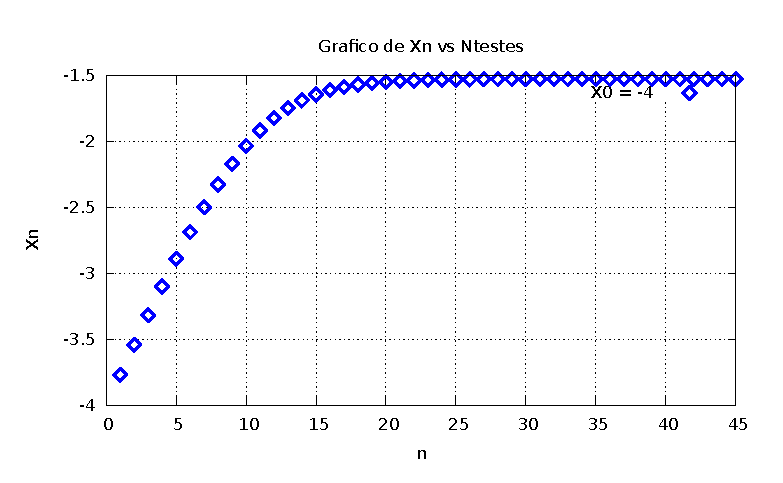
\includegraphics[width=0.5\textwidth]{grafico_do_ex01d_x=-4}
\caption{Gráfico representa o número de vezes que o programa rodou ate encontrar a raiz, para $x_0 = -4$.}
\label{ex01a1.6}
\end{figure}


\begin{thebibliography}{99}

\bibitem{Metodos} C. Scherer. Metodos Computacionais da Física (2nd ed.,2010)

\bibitem{roteiro} AULAS 9 E 10: FIS-271 - Física Computacional I

\end{thebibliography}
\end{document}